%\documentclass[11pt]{amsart}
\documentclass[review]{siamart}
\usepackage{geometry}                % See geometry.pdf to learn the layout options. There are lots.
\geometry{letterpaper}                   % ... or a4paper or a5paper or ... 
%\geometry{landscape}                % Activate for for rotated page geometry
%\usepackage[parfill]{parskip}    % Activate to begin paragraphs with an empty line rather than an indent
\usepackage{graphicx}
\usepackage{amssymb}
\usepackage{epstopdf}
\DeclareGraphicsRule{.tif}{png}{.png}{`convert #1 `dirname #1`/`basename #1 .tif`.png}
\newcommand{\Order}[1]{\ensuremath{\mathcal{O}(#1)}}    % big O notation


\title{Algorithms and software for extreme-scale particle-in-cell simulations of highly magnetized plasmas}
\author{Mark F. Adams\and Tobin Issac\and Mathew Knepley}
\nolinenumbers
\begin{document}
\maketitle

Efficient, engineering relevant, simulations of highly magnetized fusion plasmas is one of the great computational science challenges of today.
The governing equations, the Boltzmann-Maxwell system, are a set of 6D nonlinear hyperbolic equations with dynamics coupled over many decades of time and length scales.
The high dimensionality of these problems lend themselves to particle-in-cell (PIC) methods, although Eulerian methods are often at least hybridized with PIC in, for instance, the collision operator.
Additionally, the strong, complex guide fields of tokamaks generate highly anisotropic models that pose significant challenges to accurate and efficient discretizations and solvers.
Simulating highly magnetized fusion plasmas for ITER, with the accuracy and reliability necessary to be relevant to it's design and operation, is an important challenge for one of the largest scientific experiments of today.
We propose to contribution to this effort by developing efficient methods for PIC simulations in general, and for fusion plasmas in particular, and by deploying implementations optimized for emerging architectures in the PETSc numerical library \cite{}, for use by computational plasma physists.

The extreme concurrency demands of emerging architectures at extreme-scale demands careful data distribution to optimize data locality in all of the computational components and kernels of simulation codes.
This is a challenge for PIC codes because PIC methods process data in two very different data structures, which interact in particle-cell kernels such as charge deposition to the grid and particle gradient computation from the grid.
Additionally, optimal data decompositions of different computational components can be very different.
For instance, the collision operator and the deposit, solve, push phase have inherently different natural data partitionings, and the ``transpose" required to move particle between these partitions will have a cost.
Note, this is common tradeoff in computational science and can be seen in the data models used in the Eulerian fusion plasma code Gysela \cite{Gysela16}.
To this end, we focus on data distribution models for the efficient processing of particle-cell interactions and to minimize particle data communication, as well as fast solvers for, for example, Poisson's equation, Ampere's law, and the magnetohydrodymaic  solvers of implicit PIC methods \cite{DBLP:journals/cphysics/ChenC15}.
The PETSc community has extensive experience in extreme-scale solution methods for PDEs (discretizations, meshing,  nonlinear solvers, time integrators, optimization solvers, etc.) and in the deployment of optimized implementations of these methods to the public.

This document describes the support for extreme-scale PIC simulations on emerging architectures under development in PETSc.
We build on the Solver Integrated Tree-based Adaptive Refinement (SITAR) infrastructure in PETSc, for fast and accurate PDE discretizations, meshing, and solvers.
We extend SITAR with methods and features to support the development of efficient and scalable data models and algorithms for engineering relevant simulations of fusion plasmas by the computational plasma physics community.
In addition to this PETSc library work, this document describes a tokamak PIC code, X2 (\S\ref{sec:x2}).
X2 is designed from the ground up for extreme scalability and extensibility to emerging architectures.
X2 is used to drive the library development and explore the algorithmic space of modern extreme scale PIC methods, to provide data to the community on the complexities of these methods.

\section{Background}

PIC methods are popular for discretizing high dimensional problems in a variety of fields because of their low cost relative to full grid or Eulerian methods on such problems.
PIC algorithms require three types of processing: 1) particle processing (e.g., the evolution of Vlasov's equation), 2) grid processing (e.g., solvers), and 3) particle-grid interactions (e.g., particle charge deposition and gradients of potentials for particle pushing).
Pure particle processing, such as the ``push" of particles use relatively simple array processing and each particle can be processed concurrently.
Particle-grid interactions are challenging because the data structures and natural data decompositions are different, but are tightly coupled algorithmically.
The physics community has avoided much of this complexity by not decomposing field data and replicating the data on each MPI process or address space.
This data model is not tenable as we move to the exa-scale levels of parallelism required for engineering relevant ITER simulations.
Distributing grids will be very disruptive to the code base of fusion PIC applications.

%The accurate and efficient simulations of these problems, to be of engineering relevance, for say the design and operation of ITER, is an extremely challenging problem.
The physics community has developed a large body of research and experience in using PIC methods for fusion plasmas and they are one of the largest users in DOE leadership class compute facilities.
The applied math, engineering, computational science, and physics communities have developed a great deal of expertise in discretization and solver methods for extreme-scale computing, but these advanced methods are not widely used in the fusion PIC community.
The continued advancement of computational fusion physics within DOE and the global community, especially as we move from verifying computational results with theory to reliable predictive analysis, requires that both modern numerical methods and parallel computing techniques, as well as reliable software engineering methodologies, be employed.

The work proposed herein is intended to amortize both the development costs and the intellectual resources required to develop and deploy infrastructure for extreme-scale PIC applications.
This work builds on the SITAR framework in PETSc, which provides both fast solvers, tightly integrated meshing and discretizations, and optimized implementation for emerging architectures \cite{KnepleyBrownMcInnesSmithRuppAdams2015}.
SITAR is built on the highly scalable algorithms in the p4est distributed tree library \cite{DBLP:journals/siamsc/IsaacBWG15,Rudi:2015:EIS:2807591.2807675,Stadler1033}.

\section{Design Issues for Extreme-Scale PIC on Emerging Architectures}

The importance of particle-grid processing in the cost of PIC methods demands careful distribution of particles and cells to maximize data locality and minimize data movement.
Most, say well over $99\%$, of the data in a PIC simulation of a fusion devises is in the particles.
Pure grid work, such as the Poisson solver, have abundant computational resources available and, for instance, can be run entirely on the CPU of accelerated architectures, or on a reduced set of cores on symmetric systems.
However, the distribution of the grid must still be carefully designed to minimized communication cost (in the entire memory hierarchy) in particle-grid processing.
Our approach to the design of extreme-scale PIC codes is to allow for flexible particle and grid partitioning and strike an efficient balance between explicit particle communication and redundant, \Order{1}, grid storage.
This is a challenge because fusion plasma numerical methods use two distinct grids: the Poisson or Ampere's law solver grid and the collision solver grid (see Figure \ref{fig:cross}).
The optimal particle distribution for each, with respect to data locality, is very different, which results in many parameters that need to be optimized in any given algorithm.

The engineering complexity required to develop a flexible infrastructure that allows for the expression of the most optimal algorithms demands a higher level of software quality assurance processes than is often present in the codes that are driven by academic reward systems, such as number of journal publications, as opposed to the demands for reliable predictive analysis that drives the commercial sector.
%The entire software stack for a useful tokamak code may not require commercial grade software engineering, but as the size of the application code grows the level of software engineering must also grow.
Good software engineering takes both skill and time that is not available to most academic physics code projects.
PETSc employs commercial grade software engineering.
This project provides for a mechanism to provide fusion PIC codes with solid infrastructure on which to build their physics, to allow for the full use of their theoretical expertise without the demands of verifying an ever increasing software stack as we move to emerging architectures.

%The primary design principles in this work are to develop the most efficient algorithms and data decompositions for PIC processes, and to deploy them in PETSc, to develop a well engineered and verified development environment for application scientists and engineers.
%To this end, we provide a high level interface that entirely hides details of the grid, where the application scientist never touches grid entities like cells directly and instead only adds, and queries an opaque object for, data at (particle) points.
%Physicists that wish to work directly with the fields can access the grid at a lower level, but the actual data structures of the grid are always hidden.
%This allows for runtime switching between different grid types (e.g., AMR, structure, or unstructured grids can all be used transparently).
%The lowest level interface allow the user to iterate over grid entities, like cells or vertices, but hides details of the grid and discretization for maximum flexibility.
%This abstraction allows different grids, such as Cartesian, unstructured or SITAR grids to be selected at run time, without recompiling the application.

\section{General Requirements}

We have several general requirements for an extreme-scale fusion plasmas PIC application that we propose to support in PETSc and instantiate with the driver code X2 (\S\ref{sec:x2}).
\begin{itemize}
\item Flexible local grids to allow for particle-grid interaction with non-local parts of the grid.
\item Hierarchical grids for fast geometric multigrid solvers, adaptive mesh refinement, and the ``particle search" method to determine the address space of a particle.
\item Grids abstracted from application scientists to allow multiple types of grids and discretizations to be supported and selected at run time.
\item Fast nonlinear solvers for implicit PIC methods.
\item Incremental problems development for debugging and verification on Cartesian grids and ramping up to full tokamak wall geometries 
\item Finite particle form factors, or density smoothing, to allow for arbitrary mesh resolution without increasing particle count to avoid particle noise
\begin{itemize}
\item Allows decoupling grid spacing from particle form factor and facilitates AMR.
\end{itemize}
\item Multiple grid discretizations (e.g., finite volume, finite element, discontinuous Galerkin).
\item Architecture specific computational kernels for emerging architectures \cite{KnepleyBrownMcInnesSmithRuppAdams2015}.
\item Incremental contributions to the plasma physics community.
\begin{enumerate}
\item Explore different data models, collaborate with other fusion simulation projects.
\item Allow for code-to-code verification of other whole plasma ITER PIC codes.
\end{enumerate}
\end{itemize}

\section{Initial Experiments with an Extreme-Scale PIC Code for ITER Plasmas}
\label{sec:x2}

The development proposed herein takes place in a branch in the PETSc repository (mark/feature-picell) and a driver application named X2 (src/dm/impls/picell/examples/tutorials/ex1.c).
Code will likely migrate from X2 into the PETSc library as development progresses.
X2 is intended to be used to gather initial performance data on modern architectures to guide further data model developments, and to verify the PETSc library code.
Our initial approach is to exploit the fact that particle distributions, at least from a computational point of view, are relatively uniformly distributed over the domain and our grids are quasi-uniform.
This allows for particle distributions that are simply attached to cells of the solver grid, but load is balanced by using a weighted cell partitioning.
We are not, for instance, supporting multiple processes within an individual cell, but we could imagine this would be useful in the future for cosmology applications.
We currently use guide center particles only (i.e., only a parallel velocity, resulting in a 4D method) to simplify charge deposition.
These two simplifications allow us to reuse particle infrastructure that has been developed for other PETSc PIC users \cite{may2014ptatin} that attach particle to solver cells in the particle push kernel.
More complex data models with extended halo regions to accommodate gyrokinetic methods (finite shape) and high order (explicit) time integrators will be required in the near future.

The collision operator is a computational intensive nonlinear solve in velocity space on each particle collision cell.
Flux tubes are a natural choice for these collision cells, these are long, narrow subdomains that follow the twisting magnetic field lines around the torus.
We decouple the grid partitioning from the flux tube partitioning and implement a full ``transpose" of particles between these two partitions.
In the limit requires all particles be communicated at the collision frequency.
Aligning the solver partitioning with flux tubes, to minimize communication, is a potential future optimization.
%One purpose of this development is to develop performance models for PIC codes and experiment with algorithms, to base design decisions on performance models as well as data from modern machines.

Figure \ref{fig:cross} (left) shows an example of four flux tubes on a half torus and Figure \ref{fig:cross} (right) shows an example of half a coarse grid of ITER.
\begin{figure}[h!]
   \centering
   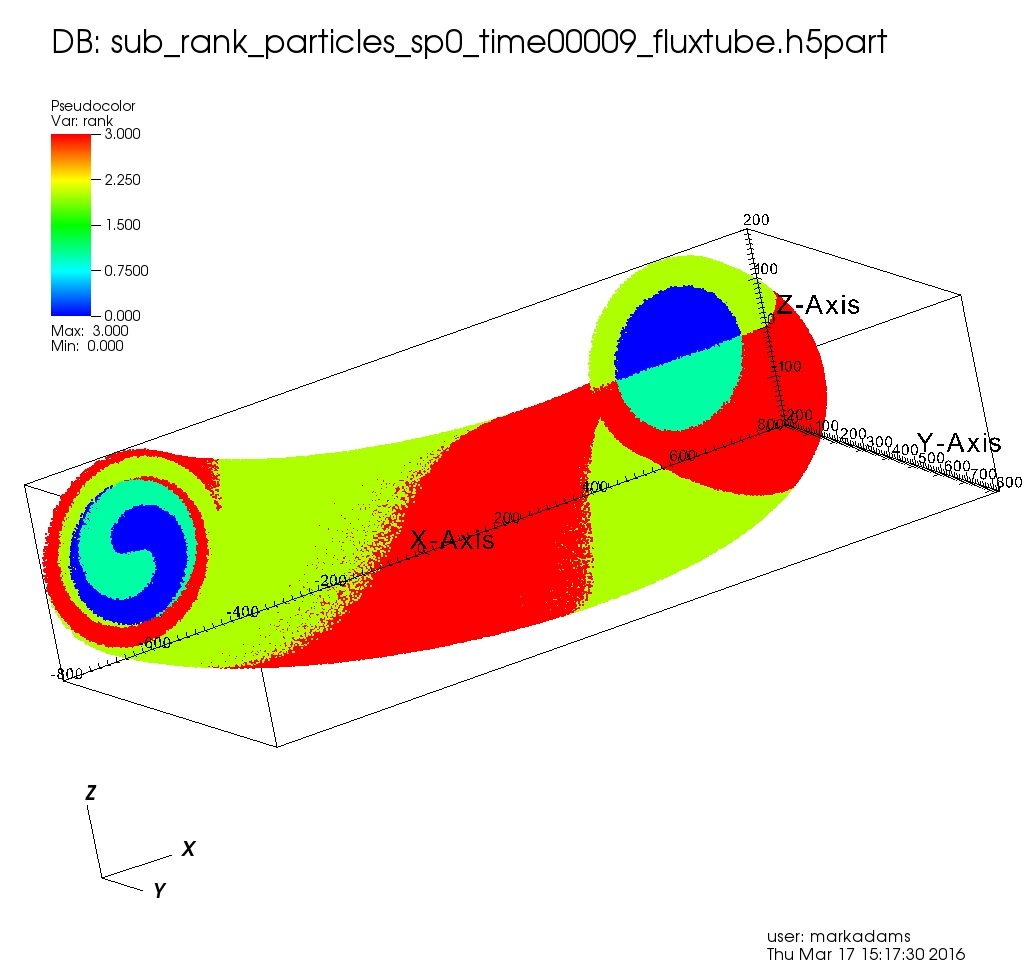
\includegraphics[width=75mm]{half_grid.jpeg} 
    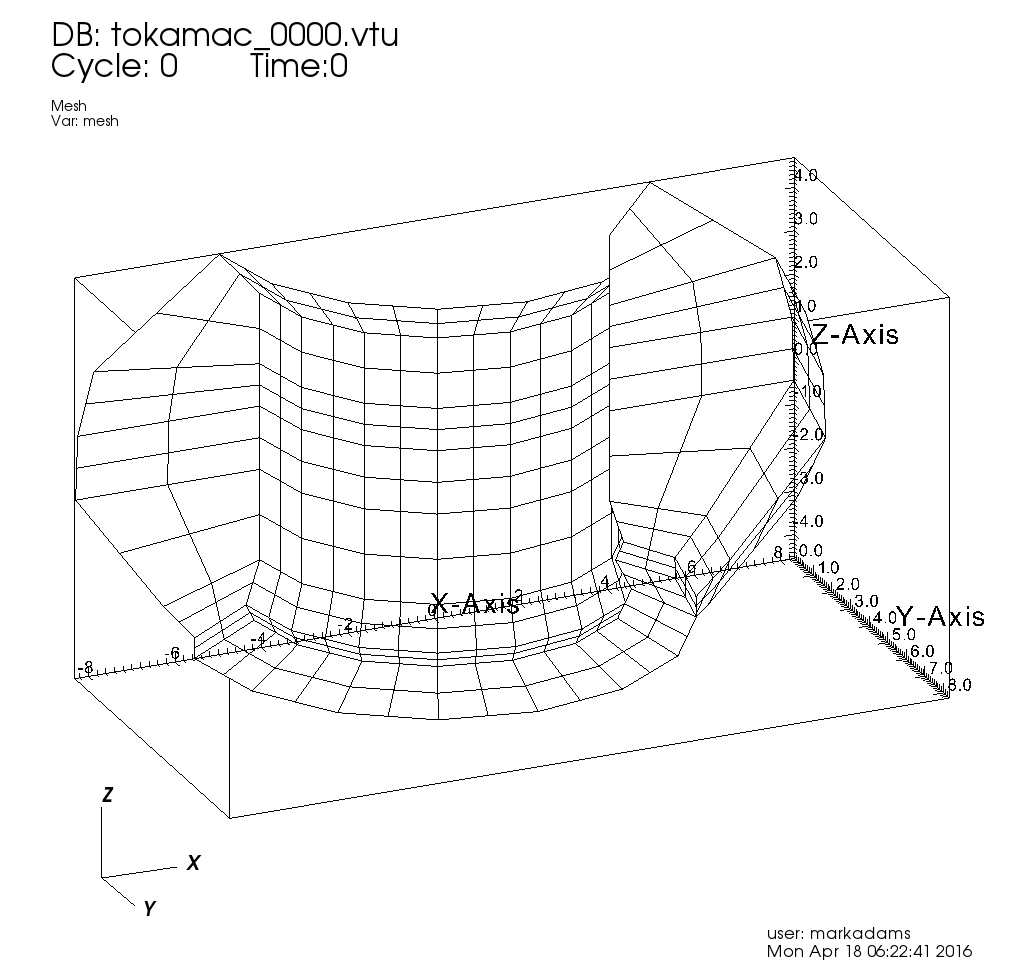
\includegraphics[width=75mm]{half_grid_mesh.jpeg} 
   \caption{Half of  2x2x2 flux tube particle partition of torus (left), corresponding coarse ITER grid solver mesh (right)}
   \label{fig:cross}
\end{figure}
The fuzzy edges of Figure \ref{fig:cross} (left) are due to the finite number of particles, each particle is drawn with the color of the partition to which it belongs.
We currently use trilinear elements, as can be seen in Figure \ref{fig:cross} (right), and intend on using Q2 elements, to resolve the domain more accurately, in the future.

In addition to equations solvers, PETSc provides advanced time integrators \cite{KnepleyBrownMcInnesSmithRuppAdams2015b}.
Fully integrating PETSc's time integrators into X2 is a long term goal.
This would require a relatively tight integration of the application with PETSc.

We plan on using Q2 finite elements in the future.
High order elements are attractive because of their high accuracy for smooth solutions and they use larger elements, because they in effect are composed of multiple ``cells" and their high accuracy allows them to be larger in physical space.
We use these elements for data locality and larger elements results in larger cell particles lists for better vectorization.
Additionally, the solutions of say the Poisson solve in fusion applications, with turbulence, are smooth at the scale of the (known) Larmore radius and, in fact, physicists often smooth the results of low order Poisson solvers to reduce noise.
We plan to move to discontinuous Galerkin (DG) methods in the future because they have attractive mathematical properties, such as having rigorous theory like finite elements and being conservative like finite volume, which would be useful for flux surface averaging projections.
DG results in systems with many degrees of freedom, a common problem of these methods, but fusion PIC solvers are highly over provisioned with processing resources, thus, local work and storage complexity are not critical for these solves.

\section{Incremental Development}

The realization of an engineering relevant full plasma simulation of ITER is a significant multi-year undertaking.
The development plans for this project are to be both incrementally relevant and engaged with the physics community.
To this end, early deliverables are important, to encourage physicists to participate with us and for us to stay grounded in the real engineering demands of this enterprise.
To this end we see several early areas that our project can contribute:
\begin{itemize}
\item Distributed data model exploration. Explore data decompositions and collect performance data to help further refine effective distributed data models for fusion PIC applications
\item Code verification. Cross code verification of existing fusion PIC codes, on somewhat simple model problems, but with full ITER wall geometries
\item Performance Verification.  Develop performance models of idioms in PIC codes (e.g., equation solvers, particle communications, particle pushing) to help application scientist verify that codes are performing correctly, by understanding the relative costs of different processes and their sensitivities (derivatives with respect to) machine metrics
\end{itemize}
 
\bibliographystyle{siamplain}
\bibliography{./bib}


 
\end{document}  